\documentclass[24pt,a0paper,portrait]{tikzposter}

\usepackage[utf8]{inputenc}
\usepackage{blindtext}
\usepackage{comment}


\title{Climate change}

\author{Ethan}
\date{\today}

\institute{University of Oxford}

%\usetheme{Board}
%
%\usetheme{Rays}
%\usetheme{Basic}
%\usetheme{Simple}
%\usetheme{Envelope}
%\usetheme{Wave}
%\usetheme{Autumn}
\usetheme{Desert}






\begin{document}

\maketitle

\block{~}
{
    Climate change includes both the global warming driven by human emissions of greenhouse gases, and the resulting large-scale shifts in weather patterns. Though there have been previous periods of climatic change, since the mid-20th century the rate of human impact on Earth's climate system and the global scale of that impact have been unprecedented.

That human activity has caused climate change is not disputed by any scientific body of national or international standing.[3] The largest driver has been the emission of greenhouse gases, of which more than 90% are carbon dioxide (CO)
2) and methane. Fossil fuel burning for energy consumption is the main source of these emissions, with additional contributions from agriculture, deforestation, and industrial processes. Temperature rise is accelerated or tempered by climate feedbacks, such as loss of sunlight-reflecting snow and ice cover, increased water vapour (a greenhouse gas itself), and changes to land and ocean carbon sinks.
}

\begin{columns}
    \column{0.4}
    \block{Causes}
    { land surfaces heat faster than ocean surfaces, deserts are expanding and heat waves and wildfires are more common. Surface temperature rise is greatest in the Arctic, where it has contributed to melting permafrost, and the retreat of glaciers and sea ice. Increasing atmospheric energy and rates of evaporation cause more intense storms and weather extremes, which damage infrastructure and agriculture. Rising temperatures are limiting ocean productivity and harming fish stocks in most parts of the globe. Current and anticipated effects from under nutrition, heat stress and disease have led the World Health Organization to declare climate change the greatest threat to global health in the 21st century. Environmental effects include the extinction or relocation of many species as their ecosystems change, most immediately in coral reefs, mountains, and the Arctic.[12] Even if efforts to minimize future warming are successful, some effects will continue for centuries, including rising sea levels, rising ocean temperatures, and ocean acidification from elevated levels of CO2
    }
    
    \column{0.6}
    \block{ Records }{ Here, Climate proxy records show that natural variations offset the early effects of the Industrial Revolution, so there was little net warming between the 18th century and the mid-19th century.[28] The Intergovernmental Panel on Climate Change (IPCC) has adopted the baseline reference period 1850 – 1900 as an approximation of pre-industrial global mean surface temperature, when thermometer records began to provide global coverage. \vspace{4cm}}
    \note[
        targetoffsetx=-9cm, 
        targetoffsety=-6.5cm, 
        width=0.5\linewidth
        ]
        {e-mail \texttt{climatechange@welfare.com}}
\end{columns}

\begin{columns}
    \column{0.5}
    \block{A figure}
    {
        \begin{tikzfigure}
            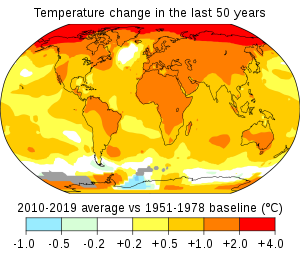
\includegraphics[width=0.4\textwidth]{./Images/change_temp.png}
        \end{tikzfigure}
    }
    \column{0.5}
    \block{Description of the figure}{ Average global temperatures from 2010 to 2019 compared to a baseline average from 1951 to 1978 }
\end{columns}

\end{document}